% BlindSpot draft 1 -- arXiv working paper (not yet submitted).
% Canonical source for the PDF; figures from make_figs.py (committed data only).
% Suggested category: cs.AI
\documentclass[11pt]{article}
\usepackage[margin=1in]{geometry}
\usepackage{graphicx}
\usepackage{amsmath,amssymb}
\usepackage{booktabs}
\usepackage{microtype}
\usepackage{hyperref}
\graphicspath{{figs/}}
\hypersetup{colorlinks=true,linkcolor=blue,citecolor=blue,urlcolor=blue}

\title{BlindSpot: Qualitative Sensing-Gap Reasoning with a Deterministic Core,\\
a Framing Model, and Hardened Verification}
\author{The BlindSpot Authors\\ \texttt{(author line placeholder for first draft)}}
\date{October 2026 (draft 1 --- field notes current to October 30, 2026)}

\begin{document}
\maketitle

\begin{abstract}
Many operational failures hide inside sensing gaps: the days a peat fire burns
under cloud, the hours a river valley is unwatched between satellite passes.
BlindSpot is a system that reasons about what such gaps may conceal. Its core
is deterministic and qualitative: detections become dated grid cells or mapped
assets, a hand-written ledger of facts is scored by frozen human weights into a
ranked set of mechanism stories, and every conclusion carries the spatial and
temporal relations it came from. A language model is allowed exactly one job ---
to frame studies and draft rival stories from anonymized evidence --- and a
default-deny verification gate decides what reaches the brief. Nothing the model
writes can move a frozen number. Two field studies carry the claim: a 2026 Nepal
flood episode, where the frozen brief named impoundment-then-burst at 0.94 and a
quarantined ground-truth window confirmed it, and a 2026 Kalimantan peat-fire
episode, where the brief named suppression-then-restart at 0.84 and both a
hidden time window and a masked half-map confirmed it. A tiered memory layer
records past episodes and stays provably silent until five labelled cases share
one pattern; a self-evolving agent may propose rule changes, test them on
held-out history, and then wait for a human. Twenty-four hardened gates enforce
all of this, and they have caught real defects --- from a shifted composition
table to a vacuous-truth hole that let empty results pass. This draft reports
the misses honestly: one-sided history, an empty flood memory, a pending flood
spatial check, and the limits of what gates can see. It closes with the
improvements that would make future demonstrations ones other systems cannot
easily copy.
\end{abstract}

\section{Introduction}
\label{sec:intro}

An operator watching a hazard --- a flood spreading down a valley, a peat fire
smouldering under haze --- rarely sees it continuously. Satellites pass
overhead on schedules of their own, clouds cover the ground for days, and
between one clear observation and the next there is a gap. The most dangerous
possibility is often the one that fits entirely inside that gap: a dam that
fails between passes, a suppressed fire that restarts under smoke. BlindSpot
exists to reason about exactly that possibility, and to do so in a way an
operator can audit down to the last arithmetic step.

Three ideas hold the system together. The first is that the reasoning should
be \emph{qualitative}. Rather than simulating water or fire physics, BlindSpot
works with relations: this region \emph{overlaps} that one, this burn period
\emph{meets} that quiet gap, this asset lies in the \emph{near} band of the
flood outline. Relations are coarser than numbers but they survive noisy
sensors, and --- crucially --- they compose: from ``the lake overlaps the
channel'' and ``the channel meets the village'' the system can derive what
must, may, or cannot hold downstream, with each step checkable by hand.

The second idea is a strict division of labour between the deterministic core
and the language model, best pictured as a measuring tape and a second doctor.
The kernel is the tape: it never stretches, never learns, so any brief can be
recomputed bit-for-bit years later. That rigidity is deliberate, and it has a
price (Section~\ref{sec:limits} records where the tape had to be amended).
The model is the second opinion in the chart: it drafts rival stories from
anonymized evidence, the brief prints its disagreement alongside the frozen
scores, and the official numbers never move toward it --- the lab results
decide the treatment, but the second opinion is on the page, not hidden. When
model and ledger disagree, as they do in both studies here, that split is the
design working, not failing.

The third idea is that verification should be mechanical, not aspirational,
because fluent machine-written code fails silently: it produces results that
look structurally perfect while being wrong. Twenty-four hardened gates run
over every change, in two different moments. Some check the code as it is
written (does every relation pair invert exactly? is builder code free of
scenario answers?). Others check the system as it runs on real data (hide all
raw inputs: does the brief come back identical? replay frozen studies: are
the bytes unchanged?). Section~\ref{sec:verification} explains both moments,
names what each caught, and admits what no gate can see.

The running picture is Figure~\ref{fig:arch}: a frozen kernel, a framing
model, a memory that mostly stays silent, and a gate that judges everything.

\begin{figure}[t]
\centering
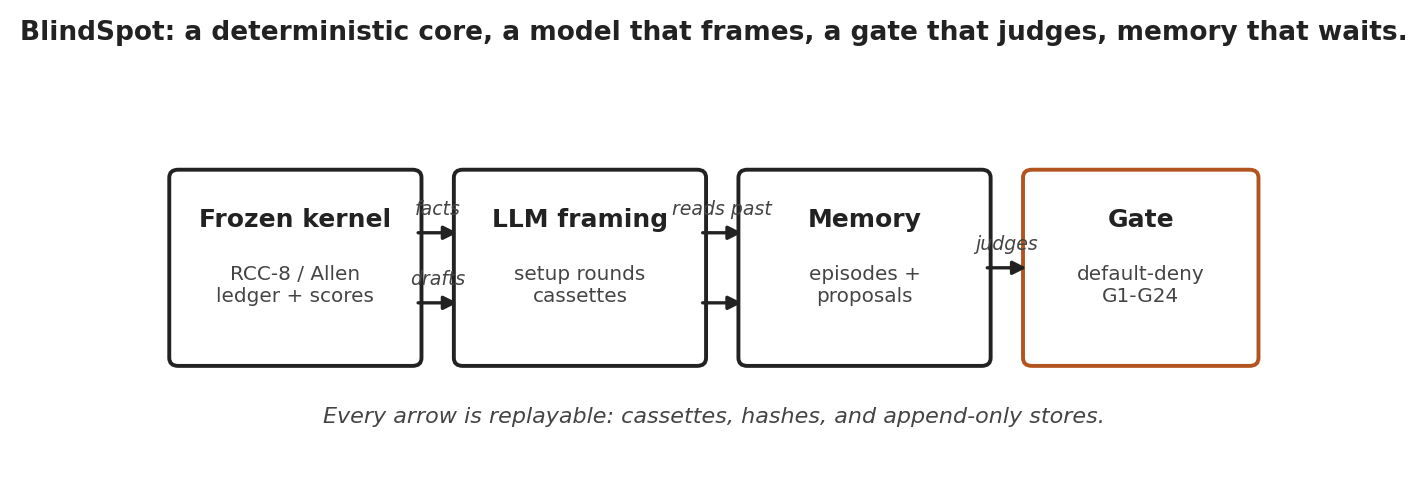
\includegraphics[width=\textwidth]{f1_architecture.png}
\caption{Four parts, one rule. The kernel never learns, the model never
scores, memory stays silent below its bar, and the gate is the only judge.
Everything the arrows carry is replayable from hashes and append-only stores.}
\label{fig:arch}
\end{figure}

\section{The core concept: what a blind spot is}
\label{sec:concept}

A \emph{blind spot} in this project has a precise meaning, and it comes in
two halves that share one cause. The cause is cloud cover, orbit schedules,
and the ordinary intermittence of satellite watching: the ground goes
unseen, and when it reappears, something may have happened in between.

The \emph{temporal} half: take two observations of the same place at two
times, $t_0$ and $t_1$. Between them lies a gap of hours or days with no
usable observation. A temporal blind spot is a physically possible event
sequence that (a) is consistent with everything seen at $t_0$, (b) is
consistent with everything seen at $t_1$, and (c) would change what an
operator should do --- a dam that fills and bursts between passes, a
suppressed fire that restarts under smoke.

The \emph{spatial} half: the same clouds hide \emph{places}, not only days.
Between a clear upstream view and a clear downstream view lies an unobserved
stretch of valley. A spatial blind spot is the ground a hidden process could
have reached unseen. The system's spatial answer is two regions: the
\emph{must-be} region (ground the process must have touched, given the
observations) and the \emph{may-be} region (ground it could have reached at
the maximum spread rate over the gap hours). Every asset of interest is then
sorted against those regions: inside must-be, inside may-be, or outside
both. That sorting is the operator's product --- it says which bridges may
be out, which power stations are exposed, which helipads remain usable.

The output vocabulary is deliberately small: the two regions, the asset
sorting, and a ranked list of mechanism stories with probabilities. In the
Nepal flood study that meant a 172.8\,km downstream may-be band, 195 exposed
assets (171 bridges, 14 hydropower facilities, 10 helipads), and six ranked
stories. In the Kalimantan fire study it meant a dated grid of burning
cells, continuity judgments between consecutive days, and four ranked
stories.

Whether the demonstrations fulfil this concept is a question we answer study
by study in Section~\ref{sec:demos}, and the honest summary is: the fire
study fulfils it twice over (two independent holdouts), the flood study
fulfils it once with the second check openly pending, and the live fire page
fulfils only the weaker claim of ``reading today,'' not prediction. A system
that cannot say which of its checks are missing is not an operator's system;
saying so is part of the design.

\section{The algebra: qualitative space and time}
\label{sec:algebra}

The kernel reasons the way a person giving directions does: not in
coordinates but in relationships --- ``the lake overlaps the channel, the
channel runs into the village, so the village is exposed.'' This section
explains the four families of relationships it uses, in plain words first and
exact conventions second. The conventions matter because half the project's
defects turned out to live in them (Section~\ref{sec:verification}): whether
``ends Monday, starts Monday'' means touching or not, whether every
comparison is checked in both directions, and which layer answers ``which
way'' when the operator asks where to look.

\subsection{The four relation families}

\paragraph{RCC-8 topology.} Given two regions, exactly one of eight
topological relations holds: disconnected (DC), externally connected (EC),
partially overlapping (PO), equal (EQ), tangential proper part (TPP) and its
inverse (TPPi), non-tangential proper part (NTPP) and its inverse (NTPPi)
\cite{randell1992}. BlindSpot classifies region pairs with exact geometric
predicates; any coordinate tolerance is applied once at ingestion from the
frozen config, never inside the classifier. Every classification is produced
in both directions, and the inverse must be the exact converse --- a property
the test suite asserts on every pair, because an early version of the
composition table had its rows shifted by a sorting mistake and every
downstream inference looked structurally fine while being wrong.

\paragraph{Allen intervals.} Given two time intervals, exactly one of thirteen
relations holds: before, meets, overlaps, starts, during, finishes, equal, and
their six inverses \cite{allen1983}. The kernel derives them from endpoints
only, on half-open day-resolution intervals, with one load-bearing rule: an
end equal to the other's start is MEETS, never BEFORE. Dates are days, not
instants, and that single convention decides whether a burn period that ends
Monday and a gap that starts Monday touch or not.

\paragraph{Rectangle algebra and tiles.} For projected extent reasoning the
kernel uses the rectangle algebra \cite{guesgen1989}: the Allen relation on
the $x$-axis paired with the Allen relation on the $y$-axis. Rectangles say
how extents overlap; they give only coarse relative position. Fine direction
--- north, northeast, bearing, ``which way to look'' --- comes from the tiles
layer beside them: each feature records which tiles of the reference's
bounding frame it touches (north, south, east, west, the four corners, and
overlap). Tiles are what the map draws; rectangles are what the reasoning
checks; together they cover orientation.

\paragraph{Bands.} Distances collapse into five preregistered bands: CONTACT
(gap of zero), IMMEDIATE\_ENVELOPE, NEAR, MEDIUM, and FAR, with the kilometre
limits frozen in configuration before any computation. A null in the config
means ``not decided'' and raises rather than defaulting --- a rule that
exists because a silent default is how scenario answers sneak into builder
code.

\subsection{Snapshot, propagation, and the gap auditor}

The kernel's central verb is \emph{snapshot}: $\mathrm{snapshot}(A,B)$ is the
relation of $A$ with respect to $B$, always computed forward
(feature-against-reference) and inverse (reference-against-feature), with the
inverse required to be the exact converse in every layer. Composition tables
let relations chain: knowing $A$-to-$B$ and $B$-to-$C$ constrains $A$-to-$C$.
The neighbourhood graph over the eight RCC-8 relations --- which relations
can transition directly into which --- is not hand-written but derived, with
witness counts stored beside it, after the generator proved that a coarse
grid made strict containment unrepresentable and forced an explicit two-scale
design with teleport jumps (DC to PO, NTPP to DC) verified absent.

The gap auditor turns these relations into the blind-spot vocabulary. From
the last-seen geometry, the gap hours, and a maximum spread rate it builds
the must-be and may-be bands; it classifies assets against them; and it runs
two detectors. Detector A (flood) tests rival upstream/downstream hypotheses
constructed from $t_0$ evidence alone --- enforced by the function signature,
which simply has no $t_1$ parameter, so reading the future is a type error
rather than a review catch. Detector B (fire) grids detections into dated
cells, audits day-to-day continuity per cell, and flags components that
vanish and reappear: the formal shape of ``suppression, then restart.''

\subsection{From facts to a ranked brief}

Each study's ledger is a small catalog of facts (six fire facts FF1--FF6 in
the Kalimantan study: run length, gap structure, clumping, and the like),
each either active or inactive for the case at hand. Human-authored rules
assign weights; each mechanism story accumulates the weights of the facts
that support it; the totals are normalized to probabilities rounded to four
places, with a largest-residual correction so they sum to exactly one (a
0.0001 surplus failed the plan's own contract once, and is now fixed in the
artifact rather than the tolerance). The frozen fire ranking is shown in
Figure~\ref{fig:rank}; the flood ranking appears in Table~\ref{tab:rankings}.

\section{What the language model does, and what it is forbidden from doing}
\label{sec:llm}

The studies in Section~\ref{sec:demos} are real 2026 emergencies: a
flood cascade in Nepal's Langtang valley and a peat-fire episode in
Kalimantan. In each case the question put to the language model was the same
one a consultant would get on day one: here is the landscape (bridges, dams,
burning grid cells) and here are the pre-cutoff facts with all names, dates,
and outcomes stripped out --- what stories could explain this, and how would
you weight them? The model's role is framing without conviction: it may
propose the stories, but the scores come from elsewhere. Given a new study, a
setup round shows the model the domain ontology and the anonymized pre-cutoff
ledger --- never names, never dates, never ground truth --- and asks it to
draft mechanism stories with weights. The round is recorded end to end:
prompts, drafts, rejections, and model-usage rows land in append-only stores,
and every model call replays offline from committed cassettes (986 model
cassettes under a 992-file manifest), so the full gate suite exercises the
neuro-symbolic path deterministically with no key and no network.

Three properties keep this honest. First, \emph{knowledge cleanliness is
tested, not assumed}: a probe asks the model about the event from anonymized
evidence, and the shipped flood probe returned ``no knowledge'' with a
self-stated cutoff predating the flood. Second, \emph{the gate is
default-deny}: every number in every model-written sentence must already
exist in the ledger's annotated numbers, with entity identifiers masked
before the scan (an early version of the rule criminalised the digits inside
\verb|bridges:7|). Anything unverified is stripped or the brief is blocked;
a skipped check counts as failure. Third, \emph{disagreement is the expected
outcome and is published}: the flood model ranked safe drainage first while
the ledger put impoundment-then-burst at 0.94; the fire model topped
\verb|smoldering_restart| against the frozen \verb|suppression_then_restart|,
yet independently weighted the same two lead facts highest (unbroken run
0.95, hotspot clumping 0.9) as the human rules. That split is the design
working: the model brings vocabulary, the frozen weights bring conviction,
and the ledger arithmetic decides. Table~\ref{tab:llm} records both
disagreements.

The setup history also contains the project's cheapest lesson in format
discipline. In an early round the model wrote short ledger identifiers while
the checker demanded full ones, producing thirty-odd citation errors; a
single instruction line fixed it permanently. A recurring failure in traces,
turned into one targeted harness change, with the evidence kept --- that is
the hill-climbing loop of Section~\ref{sec:memory} performed once by hand
before it was ever automated.

\section{The two demonstrations, and whether they fulfil the concept}
\label{sec:demos}

\begin{figure}[t]
\centering
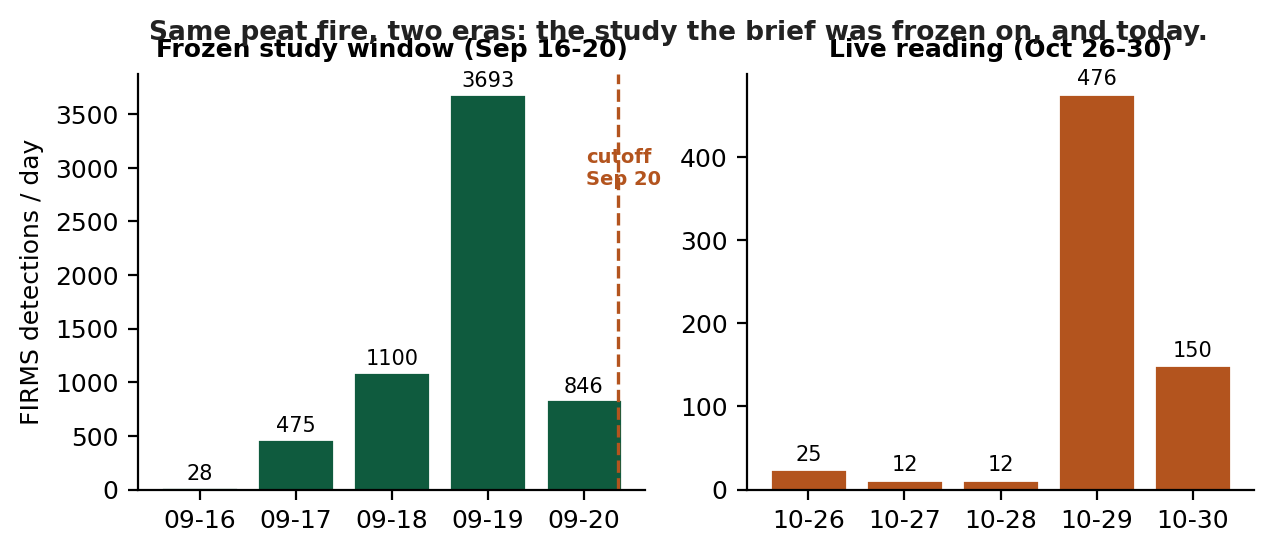
\includegraphics[width=\textwidth]{f2_fire_counts.png}
\caption{The same fire in two eras. Left: the September window the brief was
frozen on (6,142 detections over five days). Right: today's live reading
scored by the same frozen rules (675 detections, spike of 476 on October 29,
150 on October 30). The cutoff line marks what the brief was allowed to know.}
\label{fig:counts}
\end{figure}

\subsection{Kalimantan peat fire: fulfilled twice}

Peat is the fuel that lies. It burns underground, it is declared suppressed,
and then it restarts --- and the restart is the dangerous moment, because
crews have stood down. In mid-September 2026 the satellites watched a
Kalimantan peat episode through exactly this shape: 6,142 FIRMS detections
over five days (Figure~\ref{fig:counts}, left) across 30 grid cells, 28 of
them hot, with a clean multi-day gap in the middle followed by an unbroken
burn run. The frozen brief read that shape the way an experienced fire
officer would: suppression first, then peat restart --- ranked first at
0.8425 against 0.1140 for continued spread (Figure~\ref{fig:rank}, left),
before seeing anything that came after.

It was then tested the way a claim like that must be tested: twice, and
unseen both times. For the temporal check, every detection after September
20 was locked away before the brief was written; the hidden late-September
days confirmed the restart. For the spatial check, the same frozen rules
were recomputed over the western half of the map only (3,071 of 6,142
detections kept): the ranking came back identical, probabilities equal to
four decimals --- identical because scoring depends on which facts are
active, not their magnitudes. Every gate still passes on half the map, which
is itself the finding: the fire signal is spatially pervasive, not one
hotspot's doing. Figure~\ref{fig:valid} summarises all four holdout cells.

\begin{figure}[t]
\centering
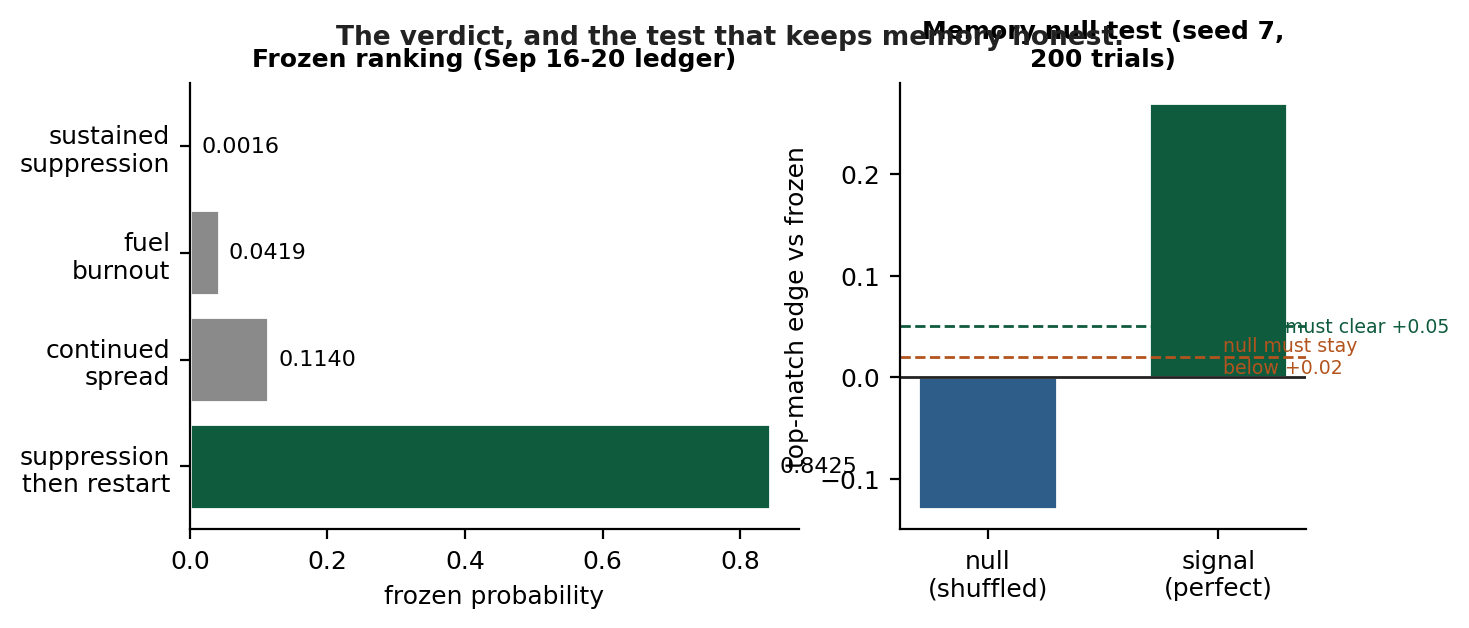
\includegraphics[width=\textwidth]{f3_ranking_null.png}
\caption{The verdict, and the test that keeps memory honest. Left: the frozen
fire ranking. Right: shuffled labels must not beat the frozen top (observed
$-0.130$, bar $+0.02$), while perfect-signal labels must gain clearly
(observed $+0.270$, bar $+0.05$). Both margins held with room to spare.}
\label{fig:rank}
\end{figure}

\begin{figure}[t]
\centering
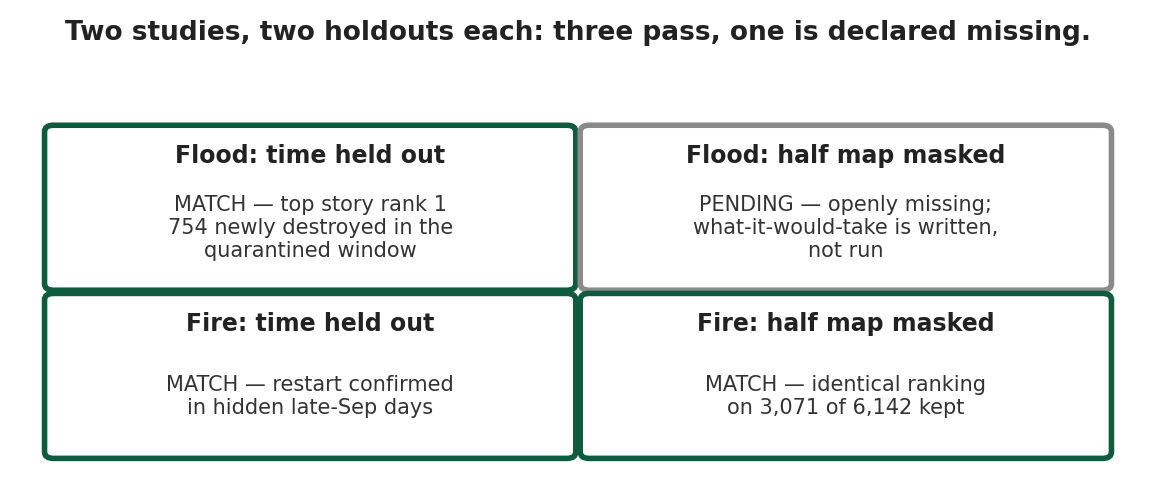
\includegraphics[width=\textwidth]{f5_validation_matrix.png}
\caption{Three of four holdout cells pass; the fourth is declared missing,
with the masked re-run specified as what-it-would-take rather than invented.}
\label{fig:valid}
\end{figure}

A live page extends the study to the ongoing fire without extending its
claims. Five October days (26--30) pulled from FIRMS under operator keys
score identically under the frozen rules, and the live signature matches the
strongest stored pattern at four labelled cases of five. The page states its
boundary on its face: this is a reading of today, not a forecast of tomorrow,
because no forecasting model exists here and none was invented. Its November
outlook is conditional arithmetic, not prediction: \emph{if} the dry regime
returns, the validated pattern restarts rather than dies out; \emph{when}
(Section~\ref{sec:postscript}) rain arrived instead, the outlook named rain
as its own falsifier in advance.

\subsection{Nepal flood cascade: fulfilled once, second check pending}

A valley floods: bad, but understood --- water comes down, bridges wash out,
crews respond. What the September 2026 Langtang-valley analysis found was a
second disaster hiding inside the first. Upstream, a secondary dam had been
impounding water behind a blockage; then it burst, and the burst multiplied
the destruction downstream far beyond what the rain alone explains. That is
the insight of this study, and it is why the stakes read the way they do:
171 bridges (no bridges, no rescue), 14 hydropower facilities (no power
stations, no power), 10 helipads (the last resort when roads are gone) ---
195 assets sorted against a 172.8\,km downstream may-be band, each one told
whether the water must have reached it or merely could have.

The frozen brief named that story --- impoundment-then-burst --- at 0.9426
(Table~\ref{tab:rankings}), before the ground truth was opened. The temporal
check then quarantined everything after the early-September cutoff and read
the hidden delta only after the freeze: 754 newly destroyed features in the
unseen window, in the channel-adjacent pattern the burst story predicts ---
a MATCH, reported as-is with no re-tuning afterward. The spatial check does
not exist yet. Flood damage exports carry almost no dates (two real damage
days against 8,368 dateless features), so no masked re-run has been
constructed; a repository-wide search verified the absence three ways before
it was declared missing rather than assumed present. That asymmetry is a
finding about the data, not the method: the flood story is confirmed in time
but untested in space, and Section~\ref{sec:future} lists exactly what would
close the gap.

\begin{table}[t]
\centering
\caption{Frozen rankings. Fire probabilities reproduce to four decimals under
the west-half mask; flood probabilities were fixed before ground truth
opened. Full mechanism titles in the study briefs.}
\label{tab:rankings}
\begin{tabular}{lll}
\toprule
Study & Mechanism & Probability \\
\midrule
Fire & suppression\_then\_restart & 0.8425 \\
     & continued\_spread & 0.1140 \\
     & fuel\_burnout & 0.0419 \\
     & sustained\_suppression & 0.0016 \\
\midrule
Flood & impoundment\_then\_burst & 0.9426 \\
      & upstream\_slope\_failure\_elsewhere & 0.0469 \\
      & downstream\_only\_flooding & 0.0082 \\
      & safe\_drainage & 0.0009 \\
      & dam\_holds & 0.0009 \\
      & no\_further\_event & 0.0005 \\
\bottomrule
\end{tabular}
\end{table}

\begin{table}[t]
\centering
\caption{The model disagrees, the ledger decides. Both disagreements are
published in the briefs; neither moved a frozen number.}
\label{tab:llm}
\begin{tabular}{lll}
\toprule
Study & Model's top story & Ledger's top story \\
\midrule
Flood & safe drainage first & impoundment-then-burst 0.94 \\
Fire & smoldering\_restart & suppression\_then\_restart 0.84 \\
\multicolumn{3}{l}{\emph{Shared:} fire model weighted the same two lead facts
highest (run 0.95, clumping 0.9).} \\
\bottomrule
\end{tabular}
\end{table}

\section{Tiered memory and the self-evolving agent}
\label{sec:memory}

Two frozen studies cannot teach a system anything --- a pattern ``seen
twice'' climbing a promotion ladder would be noise with a ceremony around it.
Memory therefore begins by manufacturing honest cases: a rolling-origin
backtest slides the cutoff across the stored fire history, runs the frozen
prediction on pre-cutoff data only, and labels the outcome with the
preregistered rule \verb|restart-noisefloor-v1| (a restart inside the window
supports the restart story; a quiet window supports the stay-out stories).
Across eleven usable scenes this yields 48 episodes, 26 of them labelled ---
all restart, because no archived scene has yet gone quiet.

Memory is four tiers. T0 is the run itself, today's ledger and brief, pinned
by hash. T1 is episodic: one append-only row per run, holding the case
fingerprint, the frozen ranking, and --- recorded later, never revised ---
the outcome and any operator verdict with its written reason. T2 is semantic:
a pattern table that is \emph{not stored at all} but recomputed on demand as
a pure function of T1, so it cannot be tampered with silently. T3 is
procedural: the rules, which change only by versioned amendment a human
approves. Reads take an \verb|as_of| date and see only episodes whose outcome
window ended before the case's own cutoff; deleting every row a case could
not have known leaves its brief byte-identical (gate G20, the memory
counterpart of the leakage gate).

A pattern's signature is a short hash over binned fact values only: gap
dictionaries project to binned day-gaps, raw floats (areas, magnitudes) leave
the key entirely, because an early key fingerprinted every slice and produced
48 patterns of one. After the approved retune, 48 patterns collapse to 22
with cross-scene grouping --- and the strongest stands at four labelled cases
against a speaking threshold of five (Figure~\ref{fig:census}). So memory
stays silent, for a verified reason rather than a promised one: with the
section absent, briefs are byte-identical to the frozen baselines (G19).

\begin{figure}[t]
\centering
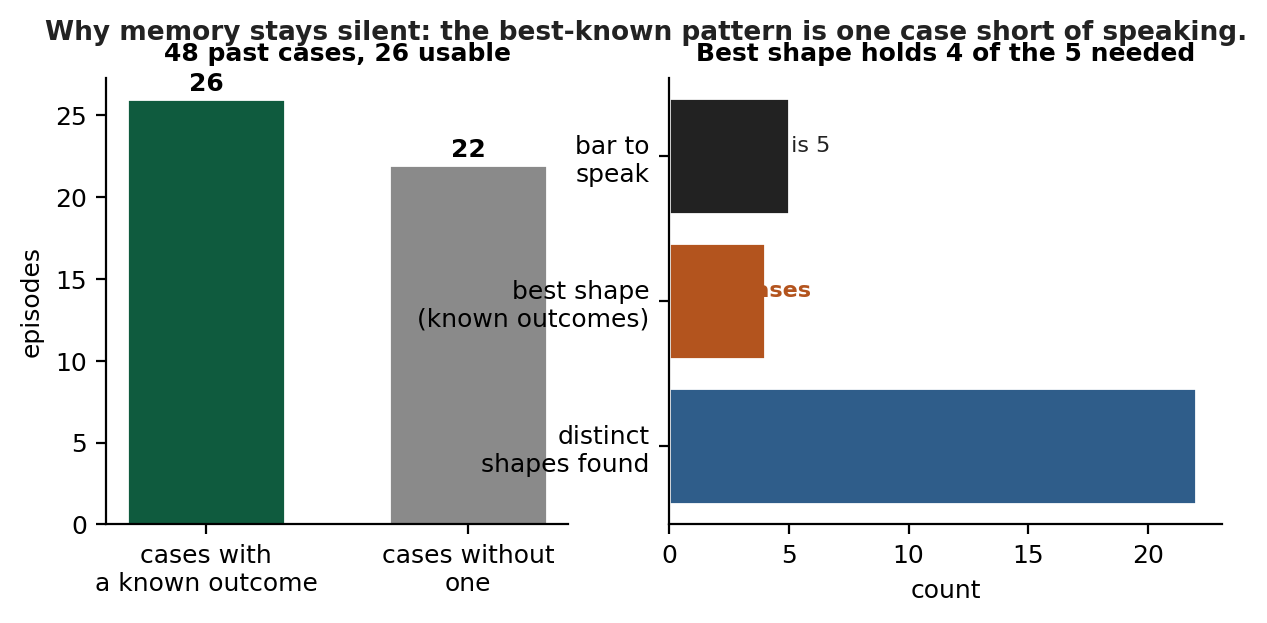
\includegraphics[width=\textwidth]{f4_census.png}
\caption{Why memory stays silent, in one chart. Left: of 48 manufactured past
cases, 26 have known outcomes (all restart). Right: they form 22 distinct
shapes, and the best-known shape holds 4 of the 5 cases the preregistered bar
requires --- one case short of speaking.}
\label{fig:census}
\end{figure}

When the bar is eventually met, the adjustment is deliberately weak. For each
mechanism, with Laplace smoothing $\alpha = 1.0$ over $n$ labelled cases:
\begin{equation}
r_m = \frac{\mathrm{hits}_m + \alpha}{n + 2\alpha}, \qquad
s_m = \mathrm{clip}(r_m - \tfrac{1}{2},\, \pm 0.10), \qquad
p'_m \propto \max(0,\, p_m + s_m),
\end{equation}
renormalized, with the frozen ranking never mutated and the shift block
printed into the ledger so the gate can check the prose against it. The null
test (Figure~\ref{fig:rank}, right) proves this math cannot manufacture skill
from noise: shuffled labels score $-0.130$ against frozen, while a
perfect-signal control gains $+0.270$. An honest side finding: once memory
speaks, long noisy histories actively hurt --- recorded as a candidate rule
fix, not a quiet retune.

The evolver --- the self-improving agent --- may propose, test, and wait. A
Proposer role with read-only tools and a hard call cap drafts single-change
proposals with cited episode and trace ids; structural checks (real ids, one
change, recurrence of at least three independent episodes) gate it through a
bounded revision loop whose feedback carries only pre-cutoff text; a Skeptic
replays the change against held-out episodes the Proposer never saw, on a
three-way time split whose final fifth is never touched during selection; and
a human approves or rejects with a written reason, with approval minting a
new version directory under a new tag. Instructions for the evolver's own
agents evolve on a separate, cheaper track that cannot alter any scientific
result. On today's data every path correctly does nothing --- no pattern
qualifies, no replay clears, and the review tool proves it by refusing ---
which is the behaviour the gates pin (G22--G24).

\begin{table}[t]
\centering
\caption{The backtest census behind Figure~\ref{fig:census}. Rule
\texttt{restart-noisefloor-v1}; two empty scene files and eleven thin-history
cutoffs skipped with printed reasons.}
\label{tab:census}
\begin{tabular}{lr}
\toprule
Item & Count \\
\midrule
Scenes slid & 11 \\
Episodes & 48 \\
Labelled (all restart) & 26 \\
Unlabelable & 22 \\
Patterns under v4 key & 22 \\
Best pattern (labelled) & 4 of bar 5 \\
Quiet scenes (mapping unexercised) & 0 \\
\bottomrule
\end{tabular}
\end{table}

\section{Hardened verification, and how useful it was}
\label{sec:verification}

The short version: the gates earned their keep, twice over --- once while
the code was being written, once while the system runs on real data --- and
Table~\ref{tab:catches} lists the receipts. The rest of this section explains
what ``hardened'' means, why the project needs it, and where its limits lie.

\begin{figure}[t]
\centering
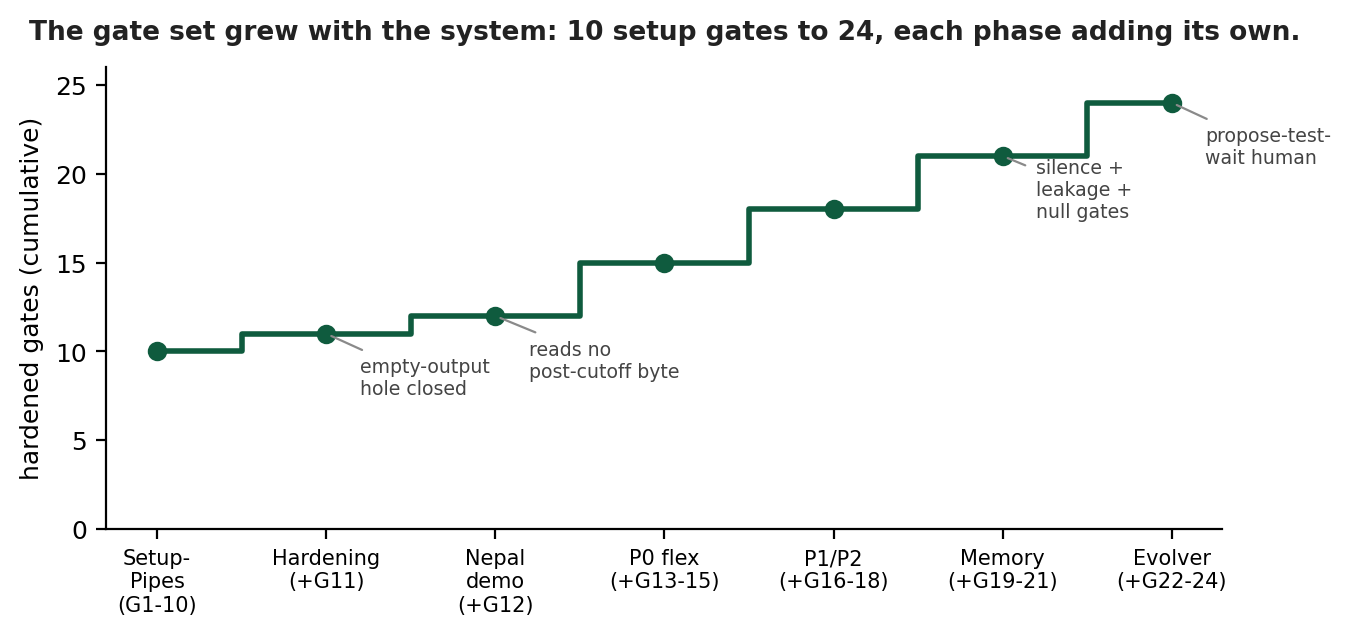
\includegraphics[width=\textwidth]{f6_gates.png}
\caption{Ten setup gates grew to twenty-four. Each phase added the gates for
its own new failure modes; the annotations mark what the additions caught.}
\label{fig:gates}
\end{figure}

\paragraph{What hardened verification is, and why it exists.} Most of this
system was written with machine assistance, and machine-written code has a
specific failure mode: it fails \emph{silently and fluently}. It produces
results that look structurally perfect --- valid tables, valid briefs, green
test suites --- while being wrong underneath. A human reviewer reading that
output nods along, because everything parses. ``Hardened'' means the checks
do not read the output the way a reviewer does; they recompute it from an
independent direction and compare. Hide all raw inputs and re-run: is the
brief byte-identical? Re-derive the scenario file from the selection rule:
is it the file the output claims? Shuffle every label: does memory still
claim skill? A gate fails closed --- a skipped check counts as failure ---
prints only claim identifiers, and the phase is not done until the full run
reports ALL PASS. An independent judge then replays the durable suite from
scratch (147 checks green at last observation).

\paragraph{The two moments: coding-time and execution-time.} The twenty-four
gates in Table~\ref{tab:gates} split into two moments, and they catch
different defects. \emph{Coding-time} checks run while the system is being
built: property tests asserting math facts the code must obey
(converse-symmetry on every relation pair, inverse snapshots everywhere),
literal scanners forbidding scenario answers in builder code, contract tests
on outputs. \emph{Execution-time} gates run the built system on real data
and demand proof: the leakage re-run with hidden inputs (G12), the frozen
replay demanding identical bytes (G14), the content-vs-input reconciliation
(G11), the memory silence/leakage/null trio (G19--G21), the restore drill
(G17). Figure~\ref{fig:gates} shows the set growing from ten setup gates to
twenty-four as each phase added the gates for its own new failure modes.

\begin{table}[t]
\centering
\caption{The hardened gate inventory. G3b is a cross-study variant of G3;
G15 covers the P0 study-gate criteria; G16--G18 cover rebuild, restore, and
ingest; G19--G24 cover memory and evolution.}
\label{tab:gates}
\footnotesize
\begin{tabular}{ll}
\toprule
Gates & What they enforce \\
\midrule
G1, G8 & Manifest discipline; input layouts conform \\
G2 & Config complete (null means undecided, never defaulted) \\
G3, G3b & No hardcoded scenario answers in builder code \\
G4, G5 & Null config exits non-zero; both pipelines exit 0 on real data \\
G6, G7 & Output contract, inverse relations, shift invariance \\
G9 & Frozen config under a git tag before any pipeline work \\
G10 & Durable suite runs inside the gate (blocking) \\
G11 & Content-vs-input: counts reconcile, scenario file reselected by rule \\
G12 & Prediction reads no post-cutoff byte; prompts quarantined and re-audited \\
G13--G15 & Cross-study genericity; frozen replay identical \\
G16 & One-command rebuild: manifest, gates, seed, API, judge \\
G17, G18 & Restore drill; raw-ingest watch \\
G19, G20 & Memory silence and memory leakage (as-of filtering) \\
G21 & Null red-team: shuffled labels must not beat frozen \\
G22, G23, G24 & Evolution discipline; loop bounds; feedback leakage \\
\bottomrule
\end{tabular}
\normalsize
\end{table}

\paragraph{What the gates caught.} Table~\ref{tab:catches} is the usefulness
ledger: each row is a real defect, the moment that caught it, and what it was
worth. Three rows deserve a sentence each. The composition-table rows were
zipped against the wrong sort order, silently shifting every row after PO;
every downstream inference looked structurally fine while being wrong, and
only the symmetry plus worked-example checks noticed --- the canonical case
for why review-style reading is not verification. The vacuous-truth hole was
worse: a structurally valid but content-empty result passed everything, so
the fix (G11) was proven on a doctored but self-consistent control built
from the wrong input file --- the exact failure the original empty-output
incident deserved. And the leakage gate caught nothing because there was
nothing to catch, which is itself evidence: hiding all raw inputs and
re-running produces byte-identical briefs, so the predictions provably read
no post-cutoff byte. The null gate's verdict --- memory loses to noise by
0.130 --- is a result, not a hurdle: it is the number that lets this paper
claim the adjustment cannot invent skill.

\begin{table}[t]
\centering
\caption{What the verification caught, and when. ``Coding'' rows broke the
build; ``execution'' rows failed a run on real data. Worth is the author's
honest grade.}
\label{tab:catches}
\footnotesize
\begin{tabular}{lll}
\toprule
Defect & Caught & Worth \\
\midrule
Composition-table rows shifted by sort order & coding: symmetry tests & very high \\
Empty result passing all structural checks & coding: G11 + doctored control & high \\
Model's short ledger ids (30+ cite errors) & coding: round rejection, 1-line fix & high \\
Post-cutoff leak search (absent, proven) & execution: G12 hide-raw re-run & high \\
Snapshot script printing ``wrote'' without writing & execution: read-back step & medium \\
Store timestamps breaking byte-stability & execution: restore drill & medium \\
Float-equality test blaming correct code & coding: fixed the test, not the code & medium \\
Prose tripping the literal scanner & coding: reworded, gate kept & low, real \\
\bottomrule
\end{tabular}
\normalsize
\end{table}

\paragraph{What plain process caught.} Not everything belongs to the gates,
and the per-phase log keeps the tags honest. The standing rules that emerged
are boring and load-bearing: execute, don't eyeball (both one-character
defects in this project were found by running, never by reading); read back
every write; never trust a check built from the assumption under test; never
weaken correct code to make a self-authored test pass.

\paragraph{What nothing here can see.} Three limits are stated openly because
they bound every claim above. First, the gates check the rule, not the
world: if the data directory itself held the wrong files, every gate would
still agree with itself; that final mile is human judgment plus the manifest.
Second, gates assert structure and bytes, not framing choices: no gate
checked the map viewport that once fitted a 172.8\,km band instead of the
feature, and prose is load-bearing in this repository down to single words.
Third, cost is real: the full suite runs just over a minute, prose scans need
tending with every new page, and each selection step against one validation
slice spends a little of that slice's honesty --- which is why the final
fifth of history is never touched during selection and is read once, at the
end, for the reported result.

The net assessment, after two studies and a memory arc: the gates were very
high value for the kernel and pipelines (where silent wrongness is cheap to
produce and expensive to notice), high value for memory and evolution (where
the failure mode is fooling oneself), and a useful tax everywhere else. A
flat result would still have been reported --- Section~\ref{sec:memory} shows
the machinery saying ``nothing qualifies'' four separate times --- and that
is the behaviour a reader should trust most.

\subsection{Postscript: the falsifier fires during drafting}
\label{sec:postscript}

On October 30, with the November outlook on the page in conditional form
(``if the dry regime returns''), news reports arrived that rain had eased the
Kalimantan fire. The rain fell after the last satellite pull, so it sits
outside every frozen number in this draft --- which is precisely the
arrangement the outlook specified: sustained rain moves the live reading out
of the restart signature, and the next pull verifies it the moment daily
counts fall. If confirmed, the quench becomes the archive's first quiet: the
fifth labelled case, the one that lets memory speak, and the first test of
the quiet mapping the labelling rule has never yet exercised. A draft that
predicts its own falsifier and then watches it arrive is either lucky or
honest; the pull CSV will decide which, and whatever it says gets recorded
as-is.

\section{Limitations}
\label{sec:limits}

A first draft is allowed cons, and this system has specific ones. The history
is one-sided: 26 restarts, zero quiets, so every learned rate is a rate of
restarting and the quiet mapping is untested code in the scientific sense.
Neighbouring backtest cutoffs overlap heavily, so episodes are not
independent no matter how the independence gap is set; the held-out splits
are strictly later in time, which mitigates but does not cure this. The
outcome rule is a proxy for truth, and operator verdicts are kept separate
from it so the proxy can later be audited rather than trusted. Flood memory
is empty for a data reason (two dated damage days against 8,368 dateless
features) that no method can argue with. The flood spatial holdout is
pending. Setup with the context card still fails its own prompt audit on real
inputs; both committed rounds ran without the card. One recorded deviation
bends the freeze discipline: the fire rules were amended after first freeze
with weights locked and outcomes accepted, counted as amendment rather than
tuning, with per-amendment rationale on file --- future studies must freeze
the learnings pass explicitly instead. And there is no forecast anywhere in
the system: every forward-looking sentence is a validated pattern pointed at
today, extended one careful step.

\section{Future work: demonstrations other systems will lack}
\label{sec:future}

Each item below ends in a demonstration that is hard to copy precisely
because it requires the machinery above to already exist.

\paragraph{The day memory speaks.} One more labelled case under the current
best pattern --- five of five --- and briefs gain a second, labelled ranking
that a null test has already proven cannot invent skill. The demo writes
itself: the same brief, before and after the fifth label, with the silence
proof and the speech proof side by side. No system without a preregistered
bar and a byte-identity silence proof can show that transition honestly.

\paragraph{Flood dated observations and the missing spatial cell.} Collecting
dated damage observations plus a preregistered flood outcome rule unlocks
both flood memory and the masked half-valley re-run. The demo is the fourth
cell of Figure~\ref{fig:valid} flipping from PENDING to MATCH (or mismatch,
reported as-is) --- a before/after no re-tuning regime can stage.

\paragraph{An evidence-strength gate.} Once memory speaks, long noisy
histories actively hurt (null $-0.130$); a gate that weighs evidence by
recency and independence, preregistered before it is measured, becomes a demo
of learning that refuses to overfit --- the rarest kind.

\paragraph{The quiet mapping.} The first archived quiet --- possibly the
October rain quench --- exercises the labelling rule's other arm, tests the
stay-out stories, and gives the Skeptic its first real replay. The demo is
memory learning that fires can end, on record.

\paragraph{Card-carrying setup rounds.} Fixing the audit alignment for card
text unblocks setup rounds that read the full redacted inventory. Fresh
cassettes, and a new prompt-hash lineage to show for the fix.

\paragraph{A third scenario, then the daemon.} A third domain (storm surge is
the natural candidate: same gap shape, different physics) proves the catalog
first. Only then does the event-driven loop earn its place: a scheduled
trigger that slides cutoffs over arriving data and starts a hill-climbing
step, with every proposal still waiting for a human. The demo is an
operator's morning brief that wrote its own audit trail overnight.

\section{Conclusion}
\label{sec:conclusion}

BlindSpot's claim is small enough to check: qualitative relations over
sensing gaps, scored by frozen weights, framed but never moved by a language
model, verified by gates that have caught real defects and state their blind
spots in writing. The fire study passes two holdouts; the flood study passes
one with the other openly pending; memory stays silent for verified reasons
and knows exactly what would let it speak; the evolver proposes, tests, and
waits. The rain that arrived during drafting gets the last word it earned:
the system named its falsifier in advance, and the next satellite pull will
say whether the pattern held. Whatever it says goes in the record as-is ---
that is the whole design, in one sentence.

\begin{thebibliography}{9}
\bibitem{allen1983} J.~F. Allen.
\textit{Maintaining knowledge about temporal intervals.}
Communications of the ACM, 26(11):832--843, 1983.

\bibitem{randell1992} D.~A. Randell, Z.~Cui, and A.~G. Cohn.
\textit{A spatial logic based on regions and connection.}
In Proc.\ 3rd Int.\ Conf.\ on Knowledge Representation and Reasoning
(KR'92), pp.\ 165--176, 1992.

\bibitem{guesgen1989} H.~W. Guesgen.
\textit{Spatial reasoning based on Allen's temporal logic.}
Technical Report TR-89-049, International Computer Science Institute,
Berkeley, 1989.

\bibitem{firms} NASA FIRMS (Fire Information for Resource Management System).
Near-real-time MODIS and VIIRS active-fire detections, distributed by NASA's
Land, Atmosphere Near real-time Capability for EO (LANCE).
\url{https://firms.modaps.eosdis.nasa.gov/}. Accessed October 2026.
\end{thebibliography}

\end{document}
